%!TeX root=../main.tex
\فصل{زبان برنامه‌نویسی پایتون}
\قسمت{مقدمه}
\begin{figure}[!h]
	\centering
	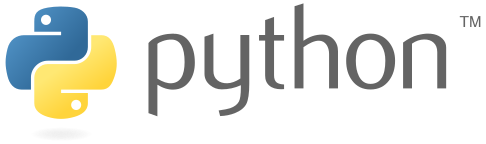
\includegraphics[width=0.7\linewidth]{Assets/python.png}
	\caption{لوگوی زبان برنامه‌نویسی پایتون.}
	\label{fig:pythonlogo}
\end{figure}

امروزه تعداد زبان های برنامه نویسی بسیار زیاد است و هر کدام کاربردهای مختلفی دارند. هر کدام از این زبان‌ها مزایا و معایب خودشان را دارند. یکی از زبان‌ های برنامه نویسی مطرح بین برنامه نویسان پایتون\پانویس{Python} است که روز به روز به میزان محبوبیت آن اضافه می شود. از این زبان برنامه نویسی برای انجام کارهایی زیادی از جمله برنامه نویسی هوش مصنوعی، توسعه وب، ساخت اپلیکیشن های موبایل و دسکتاپ استفاده می شود.

پایتون یک زبان برنامه نویسی سطح بالا تفسیر شده برای برنامه نویسی عمومی است. این زبان دارای یک فلسفه طراحی است که بر خواندن کد، به خصوص با استفاده از فضای خالی مهم استوار است. Python دارای یک سیستم نوع پویا و مدیریت حافظه خودکار است و پارادایم های چندگانه برنامه نویسی را پشتیبانی می کند. مفسر پایتون برای بسیاری از سیستم عامل ها در دسترس است.

به بیان فنی، پایتون یک زبان برنامه‌نویسی شی‌گرا\پانویس{Object-Oriented} و سطح بالا \پانویس{High-Level} با معناشناسی\پانویس{Semantic} پویای یکپارچه شده برای وب و ساخت و توسعه نرم‌افزارهای کاربردی\پانویس{Application software} است. این زبان برنامه‌نویسی در زمینه توسعه سریع نرم‌افزارهای کاربردی\پانویس{Rapid Application Development} دارای جذابیت بالایی محسوب می‌شود زیرا دارای انواع پویا\پانویس{Dynamic Types} و انقیاددهنده پویا\پانویس{Dynamic Binding} است.

پایتون، زبان برنامه‌نویسی نسبتا ساده‌ای محسوب می‌شود که یادگیری آن به دلیل دارا بودن نحو یکتایی که بر قابلیت خوانایی تمرکز و تاکید دارد آسان است. خواندن و ترجمه کدهای نوشته شده به زبان برنامه‌نویسی پایتون نسبت به دیگر زبان‌ها برای توسعه‌دهندگان\پانویس{Developers} ساده‌تر محسوب می‌شود. این موضوع به نوبه خود هزینه‌های نگهداری و توسعه برنامه‌های نوشته شده به این زبان را کاهش می‌دهد زیرا امکان همکاری تیم‌ها بدون مواجهه با موانع زبانی و وجود تجربیات کاری متفاوت در میان اعضای تیم را به دست می‌دهد.

علاوه بر این، پایتون از ماژول‌ها\پانویس{modules} و بسته‌ها\پانویس{packages} استفاده می‌کند، بدین معنا که برنامه‌های این زبان قابل طراحی به سبک ماژولار\پانویس{modular} هستند و کدهای نوشته شده در یک پروژه در پروژه‌های گوناگون دیگر نیز قابل استفاده مجدد محسوب می‌شوند. هنگامی که کاربری ماژول یا بسته مورد نیاز خود را توسعه داد، خودش یا دیگر علاقمندان (در صورتی که کد در اختیار عموم قرار بگیرد) می‌توانند آن را برای استفاده در دیگر پروژه‌ها گسترش دهند. ایمپورت\پانویس{Import} و اکسپورت\پانویس{Export} کردن این ماژول‌ها نیز کار آسانی است.

\قسمت{تاریخچه}

زبان برنامه‌نویسی پایتون در سال ۱۹۹۱ میلادی توسط یک برنامه‌نویس هلندی به‌نام خیدو فان روسوم (Guido van Rossum) ایجاد شد، این زبان با قابلیت‌های فراوان و شگفت‌انگیزی که دارد تحولی در دنیای برنامه‌نویسی به‌وجود آورده است، از توسعه‌ی برنامه‌های تحت وب گرفته تا ایجاد بازی‌های رایانه‌ای!

در سال‌های اخیر، پایتون مورد توجه بسیاری از برنامه‌نویسان بوده و روز به روز بر تعداد آن‌ها افزوده می‌شود، هرچند هنوز در ایران هنوز جایگاه خود را پیدا نکرده است، ولی می‌توان آینده‌‌‌ی روشنی برای آن تصور کرد، زیرا کاربردهای فراوانی داشته و در برنامه‌نویسی بسیاری از وبسایت‌های معتبر مورد استفاده قرار گرفته است.

پایتون یک زبان اسکریپتی است که کدهای آن در پلتفرم های لینوکس، ویندوز، مکینتاش، سیستم عامل‌های موبایل و حتی پلی‌استیشن قابل اجراست و به‌دلیل قابلیت‌های فراوانی که دارد، به یکی از زبان‌های مورد علاقه‌ی برنامه‌نویسان وب تبدیل شده و شرکت‌های بزرگی مثل گوگل، یاهو، اینستاگرام، ناسا، یوتیوب و… در سطح بالایی در حال استفاده از آن هستند.

\قسمت{ویژگی‌ها}

اولین و مهمترین ویژگی این زبان «سادگی و آسانی» آن می باشد. این ویژگی آموزش پایتون را به یکی از بهترین گزینه ها برای انتخاب کسانی تبدیل کرده است که قصد دارند برای اولین بار به آموزش برنامه نویسی بپردازند. پایتون را خیلی سریع می توانید یاد بگیرید و به سرعت کدنویسی را با آن شروع کنید. اما اشتباه نکنید، سادگی پایتون به معنای ضعیف بودن آن نیست، بلکه python یک زبان برنامه نویسی مفسری، چندمنظوره و سطح بالاست که از شی گرایی و برنامه نویسی ساختار یافته به طور کامل پشتیبانی می کند.

از این زبان برنامه نویسی به طور گسترده در دنیا استفاده می‌شود و برای آن فرقی نمی کند که هدف شما از استفاده آن ایجاد وب اپلیکیشن و برنامه نویسی دسکتاپ است و یا حتی برنامه نویسی هوش مصنوعی و یادگیری ماشینی، این زبان به بهترین نحو از عهده تمام آن ها بر خواهد آمد و به ‌جرات می‌توان ادعا کرد که در دیگر زمینه های برنامه‌ نویسی شما را تنها نخواهد گذاشت. برای اینکه بدانید که مهمترین ویژگی های پایتون چیست که آن را به چنین زبان قدرتمندی تبدیل کرده است، باید با ساختار آن آشنا شوید.

پایتون زبانی قدرتمند و منعطف است که ساختاری بسیار منظم و کدنویسی در آن بسیار راحت است. این زبان برنامه نویسی تمرکز زیادی روی خوانایی کدها دارد، به طوری که هر کسی می‌تواند به راحتی کدهای این زبان را بخواند و با آن ارتباط برقرار کند. همانطور که اشاره شد، پایتون از انواع روش‌های برنامه نویسی مثل پروسه‌ای، تابعی و البته شیء گرایی پشتیبانی می‌کند. همین مورد باعث شده که در پروژه‌های بزرگ و حساس روی پایتون حساب باز کنند.

مفسری بودن این زبان یعنی کدهای پایتون خط به خط توسط مفسر ترجمه می‌شوند. مفسر پایتون برای سیستم عامل های مختلف وجود دارد. وظیفه این مفسر تبدیل کدهای پایتون به زبان ماشین و سپس اجرای آن ها است. بسیاری از توزیع‌های لینوکس به طور پیشفرض پایتون و مفسر آن را دارند و شما بدون نیاز به انجام هیچ اقدامی می‌توانید کدنویسی را در این سیستم عامل شروع کنید. همچنین فایل نصبی نسخه ویندوز و سیستم عامل مک‌ هم از سایت پایتون قابل دانلود است.

هر نرم افزار یا ابزار جدید که معرفی می‌شود، برای انتشار از یک پروانه یا مجوز (License) استفاده می‌کند. این مجوزها ماهیت برنامه را مشخص می‌کنند و به بقیه نشان می‌دهند که چطور باید از نرم افزار استفاده کرد. مثلا نرم افزارهای آزاد ۴ سطح آزادی را به برنامه نویس تضمین می‌دهند و لایسنس GPL این چهار سطح را در خود جا داده است. ۴ سطح آزادی که نرم افزارهای آزاد باید از آن پیروی کنند عبارتند از:

کاربران بتوانند نرم افزار را به هر منظوری استفاده کنند.
کابران بتوانند نرم افزار را تغییر دهند و به سورس کد برنامه دسترسی داشته باشند.
کاربران بتوانند یک نسخه از نرم افزار را بازنشر کنند.
دیگر کاربران بتوانند نسخه‌های بازنشر شده را ویرایش کرده و دوباره انتشار دهند.
پایتون تحت پروانه اختصاصی خودش به نام PSFL یا Python Software Foundation License منتشر می‌شود. این مجوز کاملا مشابه مجوز GPL است، اما در بند چهارم سخت‌گیری کمتری برای بازنشر نرم افزارها در نظر گرفته است. به همین دلیل توسعه دهندگان به راحتی برای این زبان کتابخانه های زیادی طراحی کرده اند و به لطف آن‌ها پایتون کتابخانه‌های مشهوری دارد که در توسعه و پیشرفت آن نقش مهمی ایفا کردند. این کتابخانه‌ها بودند که پایتون را محبوب‌تر کرده و پای این زبان را به حوزه‌های مختلفی مثل طراحی سایت، طراحی اپلیکیشن، هوش مصنوعی و داده کاوی باز کردند.

\قسمت{مزایا}

حضور ماژول های شخص ثالث
Python (PyPI) شامل چندین ماژول شخص ثالث است که باعث می شود Python بتواند با بسیاری از زبان ها و سیستم عامل های دیگر ارتباط برقرار کند.\\
کتابخانه های پشتیبانی گسترده:
پایتون کتابخانه استاندارد بزرگی را ارائه می دهد که شامل موضوعات مختلف مانند پروتکل اینترنت ، عملیات رشته ، ابزارها و سرویس های وب و رابط های سیستم عامل است. بسیاری از کارهای برنامه نویسی پر کاربرد قبلاً در کتابخانه استاندارد نگاشته شده اند که باعث می شود طول کد به طور قابل توجهی کاهش داده شود.\\
منبع باز:
زبان پایتون تحت مجوز OSI تأیید شده است که استفاده و توزیع آن را آزاد می کند ، از جمله برای اهداف تجاری. علاوه بر این ، توسعه آن توسط جامعه ای انجام می شود که از طریق میزبانی کنفرانس ها، برای کد آن همکاری می کنند و ماژول های بی شماری را برای توسعه آن فراهم می کنند.\\
یادگیری سریع و آسان:
، پایگاه گسترده کاربران و توسعه دهندگان فعال باعث شده است تا یک بانک منابع اینترنتی غنی برای ترغیب توسعه و ادامه پذیرش زبان ایجاد شود.\\
ساختار داده های کاربر پسند: :
پایتون دارای ساختار داخلی داده ها و فرهنگ نامه ها است که می تواند برای ساخت سریع داده های زمان اجرا سریع استفاده شود.\\
بهره وری و سرعت:
پایتون دارای طراحی شی گرا تمیز است ، قابلیت های کنترل پیشرفته یک فرایند را فراهم می کند ، و توانایی های ادغام و پردازش متن دارد ، که همه اینها به افزایش سرعت و بهره وری آن کمک می کند. پایتون گزینه ای مناسب برای ساخت برنامه های پیچیده دارای چند پروتکل تحت شبکه محسوب می شود.

\قسمت{معایب}

سرعت:
پایتون کندتر از C یا C ++ است. پایتون یک زبان سطح بالا است ، برخلاف C یا C ++ به سخت افزار نزدیک نیست.\\
توسعه موبایل:
پایتون یک زبان خیلی خوب برای توسعه موبایل نیست. این یک زبان ضعیف برای محاسبات موبایل است. به همین دلیل است که برنامه های اندکی در تلفن های همراه مانند Carbonnelle در آن ساخته شده اند.\\
مصرف حافظه:
پایتون برای کارهای فشرده حافظه گزینه مناسبی نیست. به دلیل انعطاف پذیری انواع داده ها ، مصرف میزان حافظه پایتون نیز زیاد است.\\
دسترسی به پایگاه داده:
پایتون با دسترسی به بانک اطلاعات محدودیت هایی دارد. در مقایسه با فن آوری های رایج مانند JDBC و ODBC ، لایه دسترسی به پایگاه داده Python کمی توسعه نیافته و بدوی است.\\
خطاهای زمان اجرا:
برنامه نویسان پایتون در زمینه طراحی زبان چندین موضوع را ذکر کردند. از آنجا که این زبان به صورت پویا تایپ می شود ، به آزمایش بیشتری نیاز دارد و دارای خطاهایی است که فقط در زمان اجرا نشان می دهد.